% No specific requirements
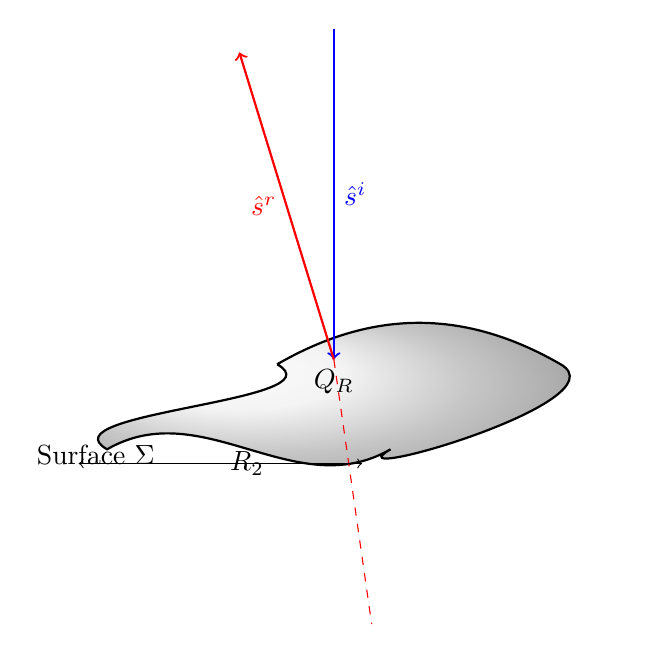
\begin{tikzpicture}[x={(-0.6cm,-0.3cm)}, y={(1cm,0cm)}, z={(0cm,1cm)}, scale=1.2]
  % Curved Surface (Convex)
  \shade[ball color=gray!20, opacity=0.6] (0,0,0) to[out=30,in=150] (0,3,0) to[out=-30,in=210] (3,3,0) to[out=210,in=30] (3,0,0) to[out=150,in=-30] (0,0,0);
  \draw[thick] (0,0,0) to[out=30,in=150] (0,3,0) to[out=-30,in=210] (3,3,0) to[out=210,in=30] (3,0,0) to[out=150,in=-30] (0,0,0);

  % Incident Ray Tube
  \coordinate (Q) at (1.5, 1.5, 0.5); % Reflection point
  \coordinate (Src) at (1.5, 1.5, 4);

  \draw[blue, ->, thick] (Src) -- (Q) node[midway, right] {$\hat{s}^i$};

  % Reflected Ray Tube
  \coordinate (Obs) at (-1, -1, 3);
  \draw[red, ->, thick] (Q) -- (Obs) node[midway, left] {$\hat{s}^r$};

  % Caustics / Virtual Focus
  \draw[dashed, red] (Q) -- (2.5, 2.5, -2);

  % Labels
  \node at (Q) [below] {$Q_R$};
  \node at (3.2, 0, 0) {Surface $\Sigma$};

  % Curvature annotations
  \draw[<->] (3.5,0,0) -- (3.5,3,0) node[midway, right] {$R_2$};
\end{tikzpicture}
